
% thesis.tex (also saved as simple.tex) -- a simple thesis document
% for demonstrating dalthesis.cls class file, or to use as a starting
% document for writing a thesis.
% If you are not familiar with TeX and LaTeX, the first thing that you
% can learn that line comments start with the percent sign (%), so
% these lines are ignored by the system.  Feel free to change them or
% delete them.
\documentclass[12pt]{report}
\newcommand{\mychapter}[2]{
    \setcounter{chapter}{#1}
    \setcounter{section}{0}
    \chapter*{#2}
    \addcontentsline{toc}{chapter}{#2}
    }
\usepackage[utf8]{inputenc}
\usepackage{graphicx}
\usepackage{gensymb}
\usepackage{comment}
\usepackage{amsmath}
\usepackage{caption}
\usepackage{subcaption}
\usepackage{pdfpages}
\usepackage[toc,page]{appendix}
\usepackage{afterpage}

\newcommand\blankpage{%
    \null
    \thispagestyle{empty}%
    \addtocounter{page}{0}%
    \newpage}
\usepackage{hyperref}

\pagenumbering{roman}

\begin{document}


% The following degrees are included in the current dalthesis.cls
% class file:
%\mcs  % options are \mcs, \macs, \mec, \mhi, \phd, and \bcshon

% If you degree is not included, you can set several options manually.
% The following example shows the parameters for the \mcs degree.
% However, if you need to set these parameters manually, please check
% the correct names with the Faculty of Graduate Studies, and let the
% maintainer of this class file know (Vlado Keselj, vlado@cs.dal.ca).
% MCS Example:





% This sample thesis contains no tables nor figures, so there is no
% need to include lists of tables and figures in the front matter:


%\frontmatter

\begin{figure}
 \centering 
 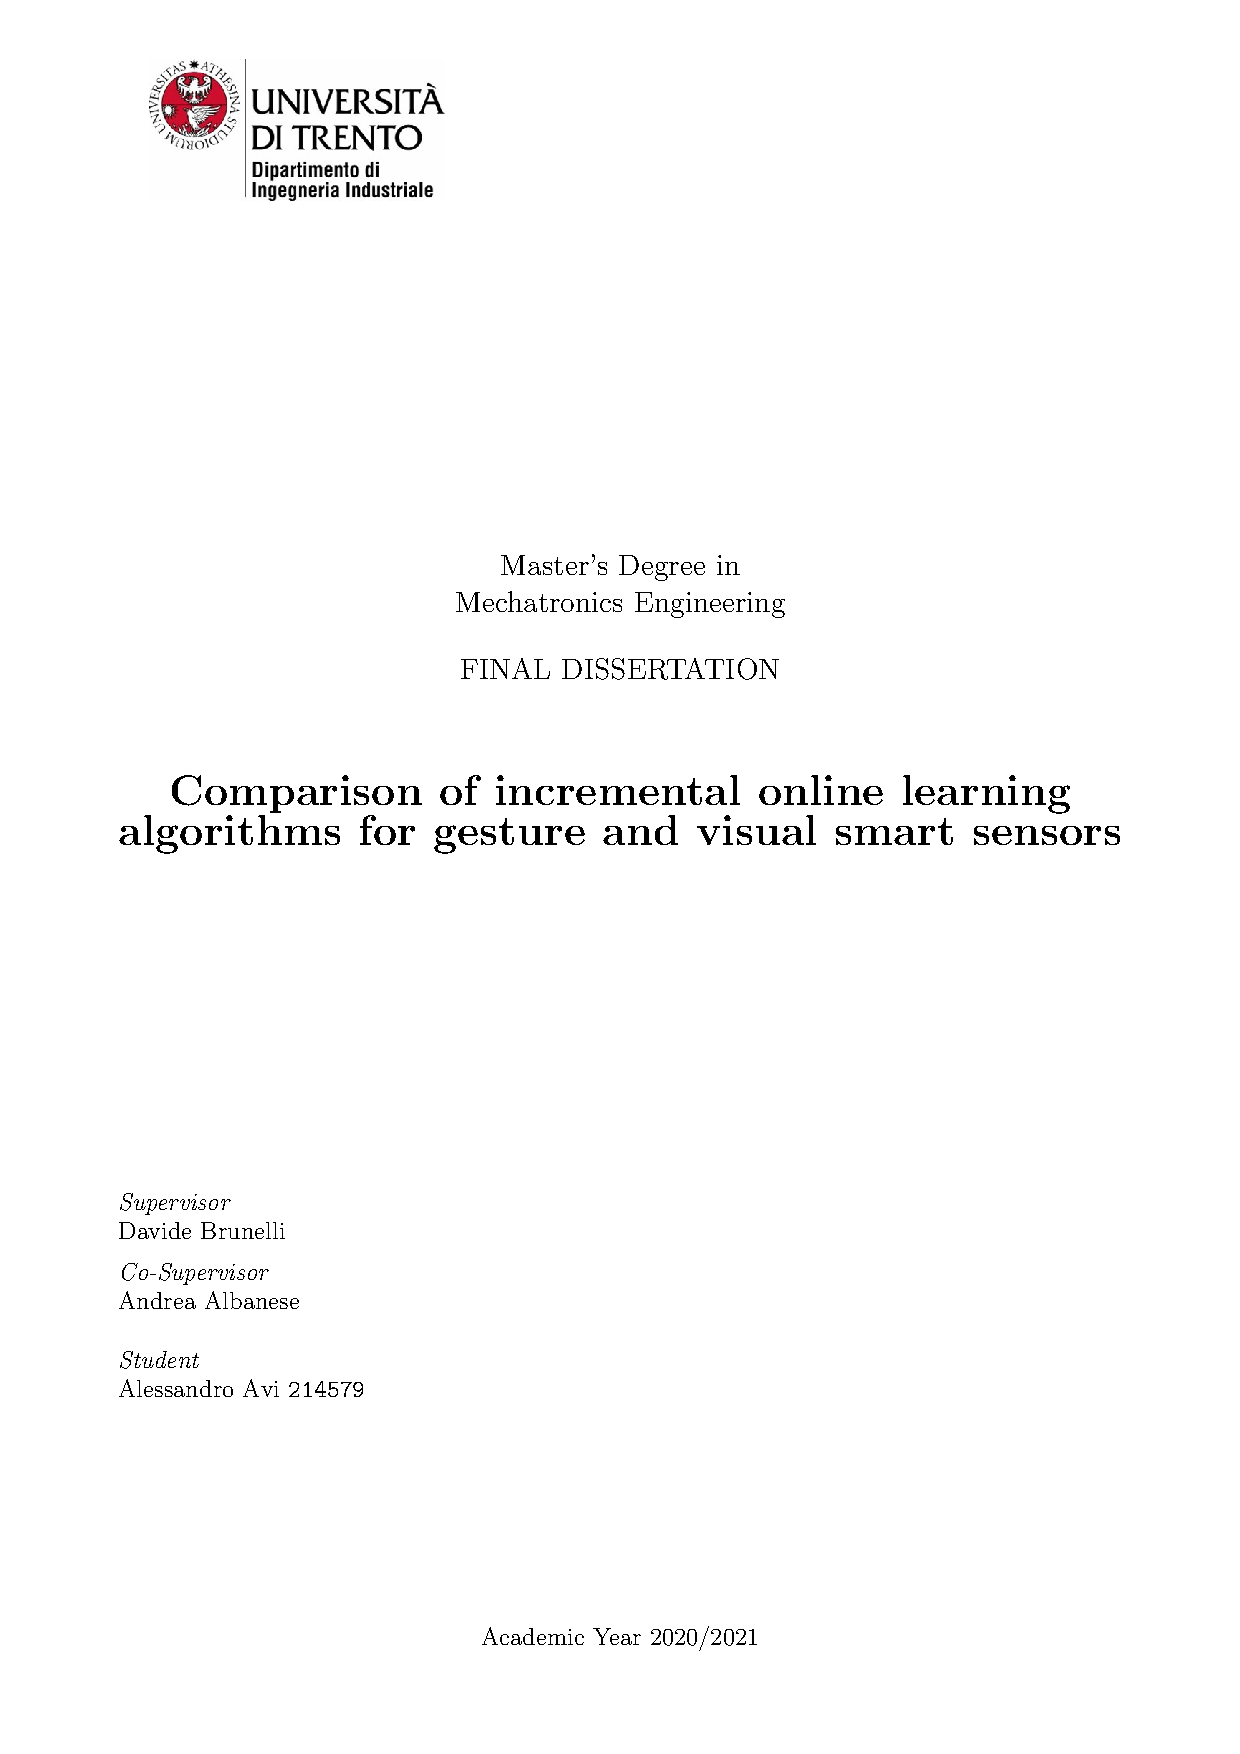
\includepdf[pages=-]{Figures/frontespizio.pdf}
\end{figure}

\afterpage{\blankpage}

\chapter*{}
\vspace*{\fill}
\textit{"There's no bad condition, only weakeness"} 
\begin{flushright}
Alex Megos
\end{flushright}
\vspace*{\fill}

\afterpage{\blankpage}





%\afterpage{\blankpage}
\tableofcontents
%\afterpage{\blankpage}
\listoffigures
\listoftables
\afterpage{\blankpage}



%\mainmatter

\mychapter{0}{Introduction}
\pagenumbering{arabic}

Application of machine learning (ML) on small devices, in a word TinyML, is becoming more and more popular as technologies advances. The usage of this type of technology on micro controllers (MCUs) is proving to be more indispensable and helpful in several applications like the industrial world, the agricultural world, autonomous driving, human machine interaction. The best field of application for TinyML is for suer the world of Internet of Things (IoT). Here machine learning finds its sweet spot since it can be exploited to change the idea of cloud computing into edge computing. The change that TinyML can bring to IoT would allow for several advantages, starting from reduced traffic on the networks and low latency for real time applications to improved security, privacy and reliability of the entire system. By exploiting all the small devices connected for performing data manipulation and elaboration, the cloud can be relieved from all the weight of computations and it could directly receive refined data already elaborated by the devices themselves. This would redirect the energy flow of all the embedded systems deployed in the environment from transmission of lots of data to elaboration of data with a subsequent transmission of high value information. By doing this the cloud is relieved from the huge amount of computation that would be required and the performances of real time application can be boosted reducing the latency. The application of edge computing brings to lots of advantages but it comes with a cost. Cost that is redirected to the preparation of intelligent MCUs, small devices that are known for their limitation in memory, computational power, limited energy sources that is strictly dependent to the limited availability of energy sources. For these reasons it's important theat the MCUs are well prepared and equipped with frameworks and systems that enabled the devicers to perform machine learning n the edge. Not only TinyML requires the correct tools for creating working fremworks but it's also required to use models specifically trained with a deployments on these devices in mind. This means generating machine learning models that are compressed and characterized by low memory and low computation power need. \\
One of the main downside of machine learning on the edge is the location of the devices in impractical locations. This can make the maintainance of the devices more difficult and resource demanding, so it's important to reduce as much as possible the maintainance on the MCUs. This is a characteristic that doesn't match with the nature of the static NN models and the natural behaviour of the enironemtn. It can be said that the NN models are incapable of adapting to the context drift that affects teh environment in which the device is deployed and the phenomenon on which data is recorded. It's in fact necesasry for these models to be frequently updated in order tomaintain a stable performance and assura reliability oer time.  





\chapter{Related Works}


\section{Machine Learning on MCU}


\section{Machine learning on edge computing}


\section{Continual-on line learning}








\chapter{Hardware} 








\chapter{Machine Learning}





\chapter{Application use cases}







\chapter{Experimental results} 






\chapter{Conclusion}





\bibliographystyle{IEEEtran}
\bibliography{thesis}

%\clearpage
%\pagenumbering{arabic}% resets page counter to 1
%\renewcommand*{\thepage}{A\arabic{page}}

%\renewcommand\appendixname{Appendix}
%\renewcommand\appendixpagename{Appendix}
%\renewcommand\appendixtocname{Appendix}

%\begin{appendices}



%\end{appendices}

\end{document}
